\documentclass[letterpaper,10pt,conference]{ieeeconf}
\IEEEoverridecommandlockouts
\overrideIEEEmargins
\usepackage{amsmath,amssymb,bm,graphicx,booktabs,array,tabularx,cite,url,xcolor,colortbl,microtype}
\usepackage[hidelinks]{hyperref}
\usepackage{listings}
\usepackage{balance}
\usepackage{capt-of}
\usepackage{mathptmx}
\renewcommand{\sfdefault}{ptm}
\renewcommand{\ttdefault}{ptm}
\setcounter{dbltopnumber}{3}
\renewcommand{\dbltopfraction}{.90}
\raggedbottom
\definecolor{plotblue}{HTML}{176B91}
\definecolor{navy}{HTML}{222222}
\definecolor{teal}{HTML}{444444}
\definecolor{orange}{HTML}{D97732}
\definecolor{softblue}{HTML}{F3F3F3}
\definecolor{softgray}{HTML}{F5F7F8}
\definecolor{codegray}{HTML}{4C5963}
\arrayrulecolor{black!65}
\renewcommand{\arraystretch}{1.10}
\setlength{\textfloatsep}{10pt plus 2pt minus 2pt}
\setlength{\floatsep}{9pt plus 2pt minus 2pt}
\setlength{\intextsep}{9pt plus 2pt minus 2pt}
\newcolumntype{Y}{>{\raggedright\arraybackslash}X}
\newcommand{\R}{\mathbb R}
\newcommand{\diag}{\operatorname{diag}}
\newcommand{\sgn}{\operatorname{sgn}}
\newcommand{\RMSE}{\operatorname{RMSE}}
\newcommand{\tablehead}{}
\newcommand{\deliverablebar}[3]{%
  \vspace{-0.35em}\noindent
  \colorbox{softblue}{\parbox{\dimexpr\columnwidth-2\fboxsep\relax}{%
    \scriptsize\color{navy}\bfseries\textsc{#1}\hfill #2\hfill #3}}%
  \par\vspace{0.45em}}
\newcommand{\widefig}[3]{\begin{figure*}[t]\centering\includegraphics[width=#2\textwidth]{figures/#1.pdf}\caption{#3}\label{fig:#1}\end{figure*}}
\newcommand{\columnfig}[3]{\begin{figure}[tbp]\centering\includegraphics[width=#2\columnwidth]{figures/#1.pdf}\caption{#3}\label{fig:#1}\end{figure}}
\newcommand{\widepng}[4]{\begin{figure*}[t]\centering\includegraphics[width=#2\textwidth]{figures/#1.png}\caption{#3}\label{fig:#4}\end{figure*}}
\lstdefinestyle{labcode}{
  basicstyle=\rmfamily\scriptsize,
  keywordstyle=\bfseries\color{navy},
  commentstyle=\itshape\color{codegray},
  breaklines=true,
  columns=fullflexible,
  showstringspaces=false,
  backgroundcolor=\color{softgray},
  frame=l,
  rulecolor=\color{teal},
  framesep=5pt,
  xleftmargin=7pt,
  aboveskip=5pt,
  belowskip=5pt
}
\lstset{style=labcode}
\newcommand{\NomRMSE}{0.0295}
\newcommand{\NomAll}{0.1146}
\newcommand{\NomMax}{0.0295}
\newcommand{\NomStart}{0.7794}
\newcommand{\NomTilt}{40.13}
\newcommand{\DragRMSE}{0.1135}
\newcommand{\DragAll}{0.1665}
\newcommand{\DragMax}{0.1135}
\newcommand{\DragStart}{0.7856}
\newcommand{\DragTilt}{40.15}
\newcommand{\CompRMSE}{0.0317}
\newcommand{\CompAll}{0.1181}
\newcommand{\CompMax}{0.0317}
\newcommand{\CompStart}{0.7820}
\newcommand{\CompTilt}{40.29}
\newcommand{\SmoothRMSE}{0.0295}
\newcommand{\SmoothAll}{0.0311}
\newcommand{\SmoothMax}{0.0295}
\newcommand{\SmoothStart}{0.0594}
\newcommand{\SmoothTilt}{7.79}
\newcommand{\SlowRMSE}{0.0344}
\newcommand{\SlowAll}{0.0641}
\newcommand{\SlowMax}{0.0344}
\newcommand{\SlowStart}{0.3717}
\newcommand{\SlowTilt}{22.27}
\newcommand{\FastRMSE}{0.2429}
\newcommand{\FastAll}{0.3763}
\newcommand{\FastMax}{0.2429}
\newcommand{\FastStart}{1.7196}
\newcommand{\FastTilt}{63.89}
\newcommand{\UnderRMSE}{0.0437}
\newcommand{\UnderAll}{0.1263}
\newcommand{\UnderMax}{0.0437}
\newcommand{\UnderStart}{0.7838}
\newcommand{\UnderTilt}{40.22}
\newcommand{\OverRMSE}{0.1049}
\newcommand{\OverAll}{0.1506}
\newcommand{\OverMax}{0.1049}
\newcommand{\OverStart}{0.7802}
\newcommand{\OverTilt}{40.36}
\newcommand{\LowRMSE}{0.0323}
\newcommand{\LowAll}{0.1674}
\newcommand{\LowMax}{0.0325}
\newcommand{\LowStart}{0.9803}
\newcommand{\LowTilt}{31.14}
\newcommand{\CompGain}{72.1}
\newcommand{\UnderGain}{61.5}
\newcommand{\OverGain}{7.5}
\newcommand{\StartGain}{92.4}
\newcommand{\YawRMSE}{5.64}
\newcommand{\HoverRMSE}{$2.10\times10^{-7}$}
\newcommand{\StepDiff}{$1.22\times10^{-12}$}
\newcommand{\PulseMax}{0.1976}
\newcommand{\PulseLate}{0.0317}
\newcommand{\FreeRad}{0.0125}
\newcommand{\FreeTan}{0.0268}
\newcommand{\FreeVert}{0.0002}
\newcommand{\UncompRad}{0.0539}
\newcommand{\UncompTan}{0.0996}
\newcommand{\UncompVert}{0.0065}
\newcommand{\ExactRad}{0.0251}
\newcommand{\ExactTan}{0.0193}
\newcommand{\ExactVert}{0.0002}
\newcommand{\JointRad}{0.0251}
\newcommand{\JointTan}{0.0193}
\newcommand{\JointVert}{0.0002}
\newcommand{\JointStart}{0.0548}
\newcommand{\JointSteady}{0.0317}
\newcommand{\JointRotor}{90.2984}
\newcommand{\JointTilt}{9.3335}
\newcommand{\DeltaPeak}{0.1982}
\newcommand{\RecoveryTime}{2.1700}
\newcommand{\JointGain}{93.0192}
\newcommand{\RosRMSESample}{0.260}
\newcommand{\RosRMSETime}{0.269}
\newcommand{\RosMax}{0.522}
\newcommand{\RosRad}{0.016}
\newcommand{\RosHeight}{0.256}
\newcommand{\RosHeightTW}{0.263}
\newcommand{\RosZMean}{1.751}
\newcommand{\RosZBias}{-0.249}
\newcommand{\RosVertShare}{96.6}
\newcommand{\RosYaw}{4.17}
\newcommand{\RosYawTW}{4.19}
\newcommand{\RosLaps}{3.02}
\newcommand{\RosSamples}{1614}
\newcommand{\RosDtMed}{0.040}
\newcommand{\RosDtMin}{0.020}
\newcommand{\RosDtMax}{0.380}
\newcommand{\MatchRMSE}{0.0114}
\newcommand{\MatchYaw}{4.30}
\newcommand{\MatchZBias}{-1.40e-05}
\newcommand{\MatchNumSlow}{0.0038}
\newcommand{\BiasUnfixed}{-0.250}
\newcommand{\BiasFixed}{-8.90e-08}
\newcommand{\BiasUnfixedRMSE}{0.250}
\newcommand{\BiasFixedRMSE}{0.0092}

\newcommand{\FlightN}{910}
\newcommand{\FlightLaps}{3.07}
\newcommand{\FlightPos}{3.0199}
\newcommand{\FlightTimePos}{2.9371}
\newcommand{\FlightMax}{9.3595}
\newcommand{\FlightRad}{1.8273}
\newcommand{\FlightHeight}{0.6227}
\newcommand{\FlightTimeHeight}{0.6001}
\newcommand{\FlightMean}{1.965}
\newcommand{\FlightBias}{-0.03458}
\newcommand{\FlightShare}{4.3}
\newcommand{\FlightYaw}{28.06}
\newcommand{\FlightTimeYaw}{27.96}
\newcommand{\FlightDt}{0.080}
\newcommand{\FlightMinDt}{0.020}
\newcommand{\FlightMaxDt}{3.340}
\newcommand{\FlightStart}{20.02}
\newcommand{\FlightEnd}{99.88}

\title{\LARGE\bf LAB3: Quadrotor Path Parameterization and\newline Geometric Trajectory Tracking}
\author{Shuyu Li\\Student ID: 24020036035\\Robot Integration Project}
\IEEEaftertitletext{%
  \begin{minipage}{\textwidth}
  \centering
  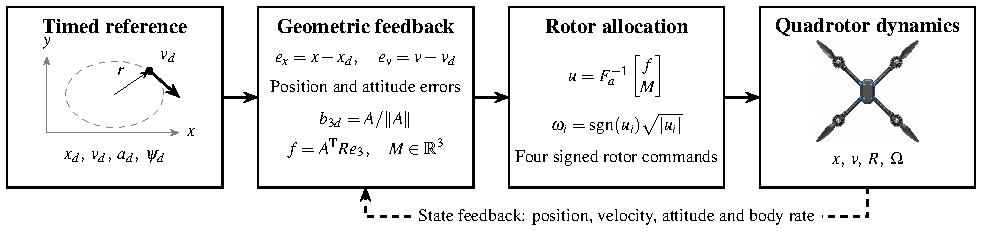
\includegraphics[width=.98\textwidth]{figures/overview.pdf}
  \captionof{figure}{Closed-loop trajectory tracking. Path timing supplies reference derivatives, geometric feedback determines force and attitude, and rotor allocation produces four motor inputs. The rigid-body state closes the feedback loop. The quadrotor illustration shows the X-layout geometry used in the allocation analysis.}
  \label{fig:overview}
  \vspace{7pt}
  \end{minipage}}
\begin{document}
\maketitle
\thispagestyle{plain}\pagestyle{plain}
\begin{abstract}
On a circular path, a quadrotor must tilt to generate centripetal acceleration while following the commanded heading. We derive the rotation conversions and rotor allocation, then evaluate a geometric controller on a 5 m-radius circle under fourteen conditions in a six-degree-of-freedom simulation. At 2.5 m/s, quadratic drag raises steady-state position root-mean-square error (RMSE) from \NomRMSE\ m to \DragRMSE\ m. Drag compensation reduces this error by \CompGain\%. With smooth startup and drag compensation, the peak startup error is \JointStart\ m and the steady-state RMSE is \JointSteady\ m. Peak rotor demand falls by 80.1\% relative to direct startup without compensation. Tangential lag accounts for most of the uncompensated error. After a lateral force pulse, the vehicle returns to within one centimeter of its unperturbed trajectory in 2.17 s. In a new official Unity flight at 1.25 m/s, the aircraft completed \FlightLaps\ laps in the evaluation window. Position RMSE was \FlightPos\ m, mean height bias was \FlightBias\ m, and yaw RMSE was \FlightYaw$^\circ$.
\end{abstract}

\section{INTRODUCTION}
\subsection{Task and Motivation}
A spatial path specifies where a vehicle should travel. A trajectory also specifies when it should reach each point, together with the required velocity, acceleration, and heading. This distinction matters for a quadrotor because horizontal acceleration requires tilting the thrust direction. A sudden change in reference velocity can therefore produce a large attitude transient even when the geometric path is smooth.

The MIT VNAV Lab 3 assignment combines rotation-representation exercises, quadrotor modeling, and geometric trajectory tracking\cite{lab}. Deliverables 1 and 2 form the individual component; Deliverable 3 covers the team controller implementation and flight validation. The circular reference provides a controlled setting in which path curvature is constant, the required centripetal acceleration is known analytically, and the influence of speed can be separated from the shape of the path.

\subsection{Questions Addressed}
The study addresses four questions. First, how should quaternion messages, rotation matrices, and angular velocities be interpreted consistently? Second, why does reversing two rotor directions remove an independent control input? Third, how does a smooth time law change startup behavior on the same circle? Fourth, how do aerodynamic drag, compensation accuracy, and feedback gains affect tracking?

The numerical comparisons use the same initial state, integration settings, and gains except when one of these is the quantity under study. Peak startup error measures how the vehicle responds as the circle begins. Steady-state error measures how closely it tracks the reference once the speed is constant.

\subsection{Experimental Approach}
Figure~\ref{fig:overview} shows the processing chain. A reference generator supplies position, velocity, acceleration, and yaw. Position feedback constructs a desired force, geometric attitude feedback aligns the body thrust axis, and a rotor-allocation matrix converts the resulting wrench into four signed rotor-speed commands. The rigid-body model returns position, velocity, orientation, and body angular velocity.

The evaluation begins with a displaced hover condition, then proceeds to direct circular tracking and smooth startup. Drag compensation is tested at the nominal speed, followed by speed variation, coefficient mismatch, and a lateral disturbance. Numerical trajectories are generated by integrating the stated equations; the ROS flight is evaluated from recorded simulator odometry. Each result table uses its corresponding state samples.

\section{ROTATION REPRESENTATIONS AND FRAME CONVENTIONS}
\deliverablebar{Individual component}{Deliverable 1}{10 pts}
\subsection{Quaternion Conversions}
ROS separates the quaternion message used for communication from the quaternion class used for computation. For the ROS 1 interfaces used by the assignment, the requested conversions are
\begin{lstlisting}[language=C++]
// Message -> tf2 quaternion
tf2::fromMsg(quat_msg, quat_tf);

// tf2 quaternion -> message
geometry_msgs::Quaternion quat_msg =
    tf2::toMsg(quat_tf);

// Scalar component and yaw
quat_tf.w();
tf2::getYaw(quat_t);
\end{lstlisting}
The first two snippets represent separate conversion tasks. The relevant conversion functions are provided by \texttt{tf2\_geometry\_msgs}; the yaw utility is available through \texttt{tf2/utils.h}\cite{tf2}.

A quaternion message can be converted to an Eigen rotation matrix as follows:
\begin{lstlisting}[language=C++]
Eigen::Quaterniond q_e(quat_msg.w, quat_msg.x,
                      quat_msg.y, quat_msg.z);
Eigen::Matrix3d R =
    q_e.normalized().toRotationMatrix();
\end{lstlisting}
The Eigen constructor takes arguments in the order $(w,x,y,z)$, whereas the ROS message fields are named $(x,y,z,w)$. Normalization is applied to a nonzero quaternion before forming the matrix\cite{eigen}.

\subsection{A Numerical Rotation Example}
For a positive $90^\circ$ rotation about the world $z$ axis,
\begin{equation}
q=(0,0,\tfrac{\sqrt2}{2},\tfrac{\sqrt2}{2}),\qquad
R=\begin{bmatrix}0&-1&0\\1&0&0\\0&0&1\end{bmatrix}.
\end{equation}
The matrix maps the body $x$ axis to the world $y$ axis, satisfies $R^TR=I$ and $\det R=1$, and yields a yaw angle of $\pi/2$. This example checks the component order, positive rotation direction, and angular unit in one calculation.

\subsection{World and Body Quantities}
Throughout the report, $R\in SO(3)$ maps a body-frame vector into the world frame. Position $x$ and linear velocity $v$ are expressed in the world frame; angular velocity $\Omega$ is expressed in the body frame. A world-frame angular-velocity measurement is therefore converted using
\begin{equation}
\Omega=R^T\omega^w.
\label{eq:omega}
\end{equation}
The same distinction is important for drag: body velocity is $v^b=R^Tv$, and a body-frame drag force is mapped back as $F_D^w=RF_D^b$. Both world and body $z$ axes point upward. This convention makes the hover check particularly simple: when $R=I$ and $v=0$, the total thrust must equal $mg$ and all three commanded moments must vanish.

\section{UAV MODELLING AND CONTROL}
\deliverablebar{Individual component}{Deliverable 2}{20 pts}
\subsection{Rigid-Body Equations}
Let $e_3=[0,0,1]^T$, let $f$ denote collective thrust along the positive body $z$ axis, and let $M$ denote the body-frame moment. The dynamics are
\begin{align}
\dot x &= v,\\
m\dot v &= -mg e_3+fRe_3+F_D^w+F_{\mathrm{ext}}^w,\label{eq:translation}\\
\dot R &= R\widehat\Omega,\\
J\dot\Omega &= M-\Omega\times J\Omega.\label{eq:rotation}
\end{align}
Here $\widehat\Omega a=\Omega\times a$. The numerical state contains position, linear velocity, a quaternion, and body angular velocity. The quaternion is integrated using body angular velocity, and its normalized rotation matrix is used in feedback.

\subsection{Full-Rank Rotor Layout}
Figure~\ref{fig:allocation} defines the rotor numbering and yaw-reaction signs. Set $a=c_fd/\sqrt2$ and $u_i=\omega_i|\omega_i|$. The collective thrust and moments satisfy
\begin{equation}
\begin{bmatrix}f\\M_x\\M_y\\M_z\end{bmatrix}
=F_a u,\quad
F_a=\begin{bmatrix}
c_f&c_f&c_f&c_f\\a&a&-a&-a\\-a&a&a&-a\\c_d&-c_d&c_d&-c_d
\end{bmatrix}.
\label{eq:allocation}
\end{equation}
For nonzero $c_f,c_d,d$, the four rows are mutually orthogonal and nonzero. Thus $\operatorname{rank}(F_a)=4$, and collective thrust, roll moment, pitch moment, and yaw moment can be assigned independently within this ideal signed-input model.

\subsection{Effect of Reversing Rotors 3 and 4}
Replacing the corresponding propellers and reversing their rotation directions preserves their upward lift convention but reverses their yaw-reaction signs. Under the numbering in Fig.~\ref{fig:allocation},
\begin{equation}
F_b=\begin{bmatrix}
c_f&c_f&c_f&c_f\\a&a&-a&-a\\-a&a&a&-a\\c_d&-c_d&-c_d&c_d
\end{bmatrix}.
\end{equation}
Its fourth row equals $-c_d/a$ times its third row. Since the first three rows remain independent,
\begin{equation}
\operatorname{rank}(F_b)=3,\qquad M_z=-\frac{c_d}{a}M_y.
\end{equation}
Pitch and yaw moments are coupled. For example, an instant requiring zero pitch moment and a nonzero yaw moment cannot be realized. Arbitrary position-and-yaw trajectories therefore cannot be tracked through four independent wrench inputs. Increasing feedback gains cannot restore this missing input direction.

\columnfig{allocation}{.98}{Illustrative top view of an X-layout quadrotor. Curved arrows indicate rotor rotation viewed from above. Labels give the rotor number and the sign of its yaw reaction moment for positive lift. In (b), reversing rotors 3 and 4 changes those signs and couples pitch and yaw allocation.}

\subsection{Feedforward Compensation for Body Drag}
For part B, compute drag from the velocity in body coordinates, rotate the estimated force into world coordinates, and subtract it from the desired thrust vector before computing the desired attitude. This supplies the opposing force as the vehicle turns. Section~\ref{sec:drag-law} gives the force law, and Table~\ref{tab:drag} compares tracking with and without compensation at the same speed.

\section{GEOMETRIC TRAJECTORY TRACKING}
\deliverablebar{Team component}{Deliverable 3}{50 pts}
\subsection{Circular Path and Analytical Derivatives}
The reference circle has radius $r=5$ m and altitude $h=2$ m. With a time-dependent phase $\theta(t)$,
\begin{align}
x_d&=[r\sin\theta,\ r\cos\theta,\ h]^T,\label{eq:path}\\
\psi_d&=-\theta,\\
v_d&=r\dot\theta[\cos\theta,-\sin\theta,0]^T,\\
a_d&=r\ddot\theta[\cos\theta,-\sin\theta,0]^T\nonumber\\
&\quad-r\dot\theta^2[\sin\theta,\cos\theta,0]^T.\label{eq:acc}
\end{align}
The desired heading follows the tangent. Uniform timing uses $\theta=t/s$, where $s$ is a time-scale parameter. The speed, centripetal acceleration, and period are
\begin{equation}
v_{\mathrm{ref}}=\frac rs,\qquad a_c=\frac r{s^2},\qquad P=2\pi s.
\end{equation}
For $s=2$ s, these values are 2.5 m/s, 1.25 m/s$^2$, and 12.57 s. The scenario is an obstacle-free prescribed path, so the planning variable studied here is its time parameterization.

Figure~\ref{fig:flight_geometry} relates the reference derivatives to the flight geometry. At constant speed, acceleration points toward the circle center and the desired heading follows the tangent. Maintaining altitude requires a vertical thrust component equal to weight, while the horizontal component supplies centripetal force.

\columnfig{flight_geometry}{.98}{Geometric interpretation of the circular reference. (a) Velocity is tangent to the path and acceleration points inward at constant speed. (b) Ideal force balance during a level turn without drag. The sketch exaggerates tilt and horizontal force for clarity. The numerical values correspond to the nominal reference.}

\subsection{Smooth Phase-Speed Transition}
A stationary vehicle begins with zero velocity. Applying uniform timing immediately creates a 2.5 m/s reference-velocity step at the nominal speed. To remove that step, a quintic phase-speed profile is used over $T=4$ s. With $\tau=t/T$ and $\omega_0=1/s$,
\begin{align}
\dot\theta&=\omega_0(10\tau^3-15\tau^4+6\tau^5),\\
\theta&=\omega_0T(\tfrac52\tau^4-3\tau^5+\tau^6),\\
\ddot\theta&=\frac{\omega_0}{T}(30\tau^2-60\tau^3+30\tau^4).
\end{align}
For $t>T$, the continuation is $\theta=\omega_0(t-T/2)$. Phase, phase speed, and phase acceleration agree at the joining time. At $t=0$, both reference velocity and acceleration are zero. Substitution into~\eqref{eq:path}--\eqref{eq:acc} preserves the circle while distributing the acceleration demand over the startup interval.

\subsection{Desired Force and Attitude}
Define position and velocity errors as $e_x=x-x_d$ and $e_v=v-v_d$. Following geometric tracking control\cite{lee}, the commanded world-frame force is
\begin{equation}
A=-k_xe_x-k_ve_v+mg e_3+ma_d-\widehat F_D^w.
\label{eq:force}
\end{equation}
The desired thrust direction is $b_{3d}=A/\|A\|$. Given the heading vector $b_{1c}=[\cos\psi_d,\sin\psi_d,0]^T$, the remaining body axes are constructed as
\begin{align}
b_{2d}&=\frac{b_{3d}\times b_{1c}}{\|b_{3d}\times b_{1c}\|},\qquad
b_{1d}=b_{2d}\times b_{3d},\\
R_d&=[b_{1d},b_{2d},b_{3d}].
\end{align}
The collective thrust is the projection
\begin{equation}
f=A^TRe_3.
\end{equation}
This projection accounts for the difference between the current and desired thrust directions. All tested trajectories have nonzero $A$ and nonparallel $b_{3d}$ and $b_{1c}$.

\subsection{Attitude Feedback and Rotor Commands}
The attitude error is
\begin{equation}
e_R=\frac12(R_d^TR-R^TR_d)^\vee.
\end{equation}
The implemented controller uses the simplified desired-angular-rate approximation $\Omega_d=\dot\Omega_d=0$, giving
\begin{equation}
M=-k_Re_R-k_\Omega\Omega+\Omega\times J\Omega.
\label{eq:moment}
\end{equation}
The rotor inputs follow from
\begin{equation}
u=F_a^{-1}[f,M^T]^T,\qquad
\omega_i=\sgn(u_i)\sqrt{|u_i|}.
\end{equation}
The orthogonal row structure of $F_a$ also gives an explicit allocation:
\begin{align}
u_1&=\frac{f}{4c_f}+\frac{M_x}{4a}-\frac{M_y}{4a}+\frac{M_z}{4c_d},\\
u_2&=\frac{f}{4c_f}+\frac{M_x}{4a}+\frac{M_y}{4a}-\frac{M_z}{4c_d},\\
u_3&=\frac{f}{4c_f}-\frac{M_x}{4a}+\frac{M_y}{4a}+\frac{M_z}{4c_d},\\
u_4&=\frac{f}{4c_f}-\frac{M_x}{4a}-\frac{M_y}{4a}-\frac{M_z}{4c_d}.
\end{align}
Collective thrust changes all four inputs equally. Roll and pitch redistribute lift between opposite sides, while yaw changes the two reaction-torque pairs in opposite directions. Substitution into~\eqref{eq:allocation} recovers the commanded wrench.

Angular speeds are expressed in rad/s. The signed square root preserves the input convention $u_i=\omega_i|\omega_i|$ used in the course model. At hover, all four speeds equal
\begin{equation}
\omega_h=\sqrt{\frac{mg}{4c_f}}=49.52\ \mathrm{rad/s}.
\end{equation}

\subsection{Quadratic Drag Compensation}\label{sec:drag-law}
The body-frame drag model is
\begin{equation}
F_D^b=-D\big(v^b\odot|v^b|\big),\qquad
D=\diag(0.1,0.1,0.2).
\end{equation}
Here $\odot$ denotes elementwise multiplication and the coefficients have units of kg/m. The force is mapped into the world frame using $F_D^w=RF_D^b$. Compensation subtracts the estimated drag in~\eqref{eq:force}; it therefore adds the force required to oppose the velocity-dependent disturbance.

With exact compensation, zero external force, and exact thrust-direction alignment, the translational error satisfies
\begin{equation}
m\ddot e_x+k_v\dot e_x+k_xe_x=0.
\label{eq:idealerror}
\end{equation}
This relation explains the role of feedforward. The simulated attitude has finite response time, so the complete closed loop retains a small periodic tracking error.

\subsection{Error Dynamics and Gain Interpretation}
The ideal relation in~\eqref{eq:idealerror} can be extended to identify the sources of residual error. Combining the commanded force with the translational dynamics gives
\begin{align}
m\ddot e_x+k_v\dot e_x+k_xe_x&=\eta,\label{eq:forcederror}\\
\eta&=(fRe_3-A)+(F_D^w-\widehat F_D^w)
+F_{\mathrm{ext}}^w.\nonumber
\end{align}
The first term is the force-direction realization error, the second is the drag-model error, and the third is the external disturbance. This decomposition connects each intervention to a physical mechanism: smooth timing moderates the rapidly changing force demand, drag compensation reduces the second term, and feedback suppresses the response to the remaining forcing.

For $\eta=0$, the energy-like function
\begin{equation}
V=\tfrac12m\|e_v\|^2+\tfrac12k_x\|e_x\|^2
\end{equation}
satisfies $\dot V=-k_v\|e_v\|^2$. Positive gains therefore give asymptotic convergence of the ideal translational subsystem. For nonzero forcing, $\dot V=-k_v\|e_v\|^2+e_v^T\eta$; sustained force error can maintain a tracking offset even though the unforced subsystem is stable.

The nominal position gains give a natural frequency of 2 rad/s and unit damping ratio. Linearizing attitude feedback near a fixed desired orientation, with $J=I$, gives a natural frequency of 10 rad/s and unit damping ratio. The attitude response is thus designed to be five times faster in this local approximation. This separation explains why the translational model is informative while finite attitude response still matters during abrupt startup and continuous turning.

\widefig{startup}{.98}{Startup comparison on the same 5 m-radius circle. The quintic phase-speed transition removes the reference-velocity step, introduces a continuous acceleration demand, and sharply reduces the initial tracking error. Each error is measured relative to that run's own time-parameterized reference.}

\section{EXPERIMENTAL DESIGN}
\subsection{Model Parameters and Integration}
Table~\ref{tab:params} gives the parameters shared across experiments. The physical constants follow the VNAV2021 controller skeleton\cite{code}; the gains are selected for that idealized model. The state is initialized with $R(0)=I$, $v(0)=0$, and $\Omega(0)=0$. Circular tracking starts at $(0,5,2)$ m, exactly on the path, so the direct-start transient is caused by velocity and acceleration demands rather than an initial position offset.

The differential equations are integrated with DOP853, a maximum step of 0.02 s, relative tolerance $10^{-9}$, and absolute tolerance $10^{-11}$. Each run lasts 30 s and is sampled every 0.01 s, yielding 3001 state records. Feedback is recomputed at the integration stages. The force-pulse run is split at its switching times, 12 and 13 s, to resolve the input discontinuities.

The experiments use exact state feedback and ideal signed rotor inputs, with no motor lag or saturation. The results describe continuous-feedback rigid-body simulation under these assumptions.

\begin{table}[t]
\caption{Shared numerical parameters}\label{tab:params}\centering\small
\begin{tabular}{@{}ll@{}}\toprule
\tablehead Quantity & Value\\\midrule
Mass $m$ & 1 kg\\
Gravity $g$ & 9.81 m/s$^2$\\
Inertia $J$ & $I_3$ kg\,m$^2$\\
Rotor arm length $d$ & 0.3 m\\
Lift coefficient $c_f$ & $10^{-3}$ N\,s$^2$\\
Yaw coefficient $c_d$ & $10^{-5}$ N\,m\,s$^2$\\
Position / velocity gains & $k_x=4$, $k_v=4$\\
Attitude / rate gains & $k_R=100$, $k_\Omega=20$\\
Nominal radius / height & $r=5$ m, $h=2$ m\\
Nominal time scale & $s=2$ s\\
Smooth-start duration & $T=4$ s\\
Simulation / record interval & 30 s / 0.01 s\\\bottomrule
\end{tabular}
\end{table}

\subsection{Metrics and Evaluation Windows}
For a sampled trajectory, define $e_i=\|x(t_i)-x_d(t_i)\|_2$. The position root-mean-square error is
\begin{equation}
\RMSE=\sqrt{\frac1N\sum_{i=1}^N e_i^2}.
\end{equation}
The maximum error over $0\le t\le4$ s measures startup response. Steady-state RMSE and maximum error are computed over $10\le t\le30$ s, containing 2001 samples. Full-run RMSE includes all 3001 samples. Tilt is $\cos^{-1}(e_3^TRe_3)$, and yaw error is wrapped to $[-\pi,\pi]$ before its RMSE is computed.

To distinguish geometric deviation from progress along the path, define the outward radial and forward tangential directions
\begin{equation}
n_r=[\sin\theta,\cos\theta,0]^T,\qquad
n_t=[\cos\theta,-\sin\theta,0]^T.
\end{equation}
The signed error components are $e_r=n_r^Te_x$, $e_t=n_t^Te_x$, and $e_z=e_3^Te_x$. Positive $e_r$ points outward and positive $e_t$ indicates a displacement ahead of the reference tangent. Their orthonormal construction gives
\begin{equation}
\RMSE^2=\RMSE_r^2+\RMSE_t^2+\RMSE_z^2.
\label{eq:components}
\end{equation}
The projections describe displacement from the instantaneous reference point; the exact horizontal distance from the circle is $|\sqrt{x_1^2+x_2^2}-r|$.

Each deterministic comparison uses a common evaluation window. Single-factor runs measure the effect of each change. The combined run tests smooth timing and drag compensation together.

\subsection{Experiment Matrix}
Table~\ref{tab:experiment_matrix} groups the fourteen numerical conditions by the question each comparison addresses. The nominal circle supplies the shared baseline. The hover target is $(0,5,2)$ m and its initial position is $(0.5,4.5,1.5)$ m. All drag comparisons use the same true matrix $D$, while the estimated matrix is $\widehat D=\alpha D$.

\begin{table}[tbp]
\caption{Numerical experiment matrix. Counts sum to fourteen distinct conditions. Shared baselines are counted once.}\label{tab:experiment_matrix}
\centering\footnotesize\setlength{\tabcolsep}{3pt}
\begin{tabularx}{\columnwidth}{@{}lYr@{}}
\toprule
Study & Conditions and purpose & Runs\\\midrule
Hover & Displaced initial state, equilibrium check & 1\\
Startup & Nominal, smooth timing and lower $k_v$, transient response & 3\\
Attitude gains & Lower $k_R$ and higher $k_\Omega$, heading lag & 2\\
Drag & Uncompensated and exact compensation, steady offset & 2\\
Speed & Slower and faster circles, speed dependence & 2\\
Model mismatch & Half and excess drag compensation, coefficient sensitivity & 2\\
Combined design & Smooth timing with exact compensation, joint performance & 1\\
Disturbance & Lateral pulse on the combined design, recovery & 1\\\midrule
Total & Shared model and evaluation definitions & 14\\
\bottomrule
\end{tabularx}
\end{table}

The attitude-gain comparison uses $(k_R,k_\Omega)=(100,20)$, $(50,20)$, and $(100,40)$ with direct timing and no drag. The speed comparison uses $s\in\{4,2,1\}$ s, corresponding to 1.25, 2.5, and 5 m/s. The model-mismatch comparison uses $\alpha\in\{0,0.5,1,1.5\}$. The disturbance experiment uses smooth startup, exact drag compensation, and a 1 N world-frame $x$ force from 12 to 13 s. The combined design also provides the unperturbed baseline for the pulse experiment. A separate nominal run with the maximum integration step halved checks numerical consistency.

\columnfig{hover_rotors}{.98}{Hover convergence and nominal circular-flight inputs. (a) Position errors from an initial displacement of $(0.5,-0.5,-0.5)$ m. (b) Signed rotor-speed commands during direct circular startup. Negative values are part of the ideal signed-input model specified in the methods.}

\section{RESULTS}
\subsection{Hover Convergence and Input Scale}
The hover errors in Fig.~\ref{fig:hover_rotors} decay from the initial displacement toward zero. The steady-state position RMSE is \HoverRMSE\ m, with an initially zero desired velocity and acceleration. This result checks the gravity sign, the body-to-world transformation, and the zero-moment equilibrium.

The rotor commands reveal the cost of an abrupt circular start. The largest absolute command is 453.91 rad/s for direct startup, compared with 91.36 rad/s for smooth startup. These values exceed the 49.52 rad/s hover speed because the ideal model must also generate moments during the initial reorientation. Smoothing the reference therefore reduces both position error and peak input demand.

\subsection{Nominal Circular Tracking}
Figure~\ref{fig:circle} shows the reference and simulated trajectories. After the initial transient, the tracked position closely follows the prescribed circle. The 30 s nominal reference covers approximately 2.39 revolutions. Full-run position RMSE is \NomAll\ m, decreasing to \NomRMSE\ m over the steady-state window. The steady-state maximum error is \NomMax\ m.

The time histories in Fig.~\ref{fig:tracking} explain the difference between those two metrics. The reference begins with a nonzero tangential velocity, producing an early error peak; afterward, the position error becomes a small periodic response. The three-dimensional plot magnifies the altitude axis to show the transient vertical excursion, while the top view preserves the circular geometry.

\subsection{Startup Timing and Velocity Damping}
Table~\ref{tab:startup} compares two timing laws and two velocity gains. Smooth startup reduces the maximum error in the first 4 s from \NomStart\ m to \SmoothStart\ m, a \StartGain\% reduction. Peak tilt falls from \NomTilt$^\circ$ to \SmoothTilt$^\circ$. The steady-state errors remain almost identical because both timing laws eventually reach the same constant phase speed.

Reducing $k_v$ from 4 to 2 increases the direct-start peak from \NomStart\ m to \LowStart\ m and full-run RMSE from \NomAll\ m to \LowAll\ m. The ideal translational model in~\eqref{eq:idealerror} has natural frequency $\sqrt{k_x/m}=2$ rad/s and damping ratio $k_v/(2\sqrt{mk_x})$. The corresponding ratios are 1 and 0.5. The more oscillatory response at the lower gain agrees with this interpretation, while the full simulation also includes attitude dynamics.

\columnfig{circle}{.98}{Nominal circular tracking without drag. The dashed curve is the reference and the solid curve is the integrated vehicle trajectory. The point labeled Start marks the initial position. The altitude range in the three-dimensional view is expanded to reveal the small vertical transient.}

\begin{table}[tbp]
\caption{Timing and damping comparison without drag}\label{tab:startup}\centering\footnotesize\setlength{\tabcolsep}{2.6pt}
\begin{tabularx}{\columnwidth}{@{}Yrrrr@{}}\toprule
\tablehead Condition & \shortstack{Full RMSE\\(m)} & \shortstack{Steady RMSE\\(m)} & \shortstack{Start max.\\(m)} & \shortstack{Peak tilt\\($^\circ$)}\\\midrule
Direct start, $k_v=4$ & \NomAll & \NomRMSE & \NomStart & \NomTilt\\
Direct start, $k_v=2$ & \LowAll & \LowRMSE & \LowStart & \LowTilt\\
Smooth start, $k_v=4$ & \SmoothAll & \SmoothRMSE & \SmoothStart & \SmoothTilt\\\bottomrule
\end{tabularx}
\end{table}

\subsection{Heading Lag under Simplified Attitude Feedback}
The nominal steady-state yaw RMSE is \YawRMSE$^\circ$. Equation~\eqref{eq:moment} damps the actual angular rate toward zero even while the reference heading keeps rotating. A persistent attitude error is therefore needed to balance the damping term.

For a near-level vehicle undergoing approximately pure yaw, this balance gives
\begin{equation}
k_R\sin\delta\approx k_\Omega|\dot\psi_d|.
\end{equation}
With $k_R=100$, $k_\Omega=20$, and $|\dot\psi_d|=0.5$ rad/s, it predicts $\delta\approx\sin^{-1}(0.1)=5.74^\circ$, close to the measured \YawRMSE$^\circ$. The small difference reflects the tilted three-dimensional motion. This calculation shows why accurate position tracking can coexist with a visible heading lag.

\subsection{Matched Attitude-Gain Experiments}
The heading-lag prediction is tested by changing one attitude gain at a time while keeping the trajectory and translational gains fixed. Table~\ref{tab:attitude} compares the measured yaw RMSE with the near-level prediction. Halving $k_R$ or doubling $k_\Omega$ doubles the ratio $k_\Omega/k_R$. Both changes raise the predicted lag from $5.74^\circ$ to $11.54^\circ$, and the two simulations give approximately $11.35^\circ$. The prediction differs from the measured value by less than $0.20^\circ$ in all three cases.

The gain changes also increase steady position RMSE from 0.0295 m to approximately 0.0593 m. For a fixed desired attitude, the local characteristic equation is $\lambda^2+k_\Omega\lambda+k_R=0$. The nominal poles are $-10,-10$ s$^{-1}$. Reducing $k_R$ gives $-17.07,-2.93$ s$^{-1}$, while increasing $k_\Omega$ gives $-37.32,-2.68$ s$^{-1}$. Both alternatives introduce a slower dominant mode. Thus, greater rate damping can slow force-direction tracking even as it suppresses rapid rotational motion.

Figure~\ref{fig:tracking}(d) distinguishes this gain-dependent heading offset from the position-loop oscillation in panel (b). The experiments support tuning position damping and attitude response separately: $k_v$ shapes translational settling, whereas $k_R$ and $k_\Omega$ jointly determine orientation response and the persistent lag under the simplified rate law.

\begin{table}[tbp]
\caption{Attitude-gain comparison: analytical heading lag and simulated tracking}\label{tab:attitude}\centering\footnotesize\setlength{\tabcolsep}{2.6pt}
\begin{tabularx}{\columnwidth}{@{}Yrrrrr@{}}\toprule
\tablehead Condition & $k_R$ & $k_\Omega$ & \shortstack{Pred. lag\\($^\circ$)} & \shortstack{Yaw RMSE\\($^\circ$)} & \shortstack{Pos. RMSE\\(m)}\\\midrule
Nominal & 100 & 20 & 5.74 & 5.64 & 0.0295\\
Lower attitude gain & 50 & 20 & 11.54 & 11.35 & 0.0593\\
Higher rate damping & 100 & 40 & 11.54 & 11.35 & 0.0593\\
\bottomrule\end{tabularx}

\end{table}

\widefig{tracking}{.96}{Position and attitude tuning on the same circular reference without drag. (a) Nominal world-frame position error. (b) Position-error norm for two velocity gains. (c) Nominal vehicle tilt. (d) Wrapped yaw error for three attitude-gain settings. Doubling the rate-to-attitude gain ratio approximately doubles the sustained heading offset.}

\columnfig{gain_diagnosis}{.98}{Attitude-gain diagnosis using the saved gain-study results. (a) Roots of the local characteristic equation. The pole closest to zero determines the slowest local mode. (b) Near-level heading-lag prediction compared with steady-state yaw RMSE. Both modified gains introduce a slower mode and approximately double heading lag.}

Figure~\ref{fig:gain_diagnosis} combines the local dynamic prediction with the measured heading error. All three gain settings have stable local poles. Their different distances from zero explain why increasing angular-rate damping can produce a slower response. The heading-lag prediction agrees with the measured yaw RMSE within $0.20^\circ$ for all three settings.

\subsection{Drag Compensation at Matched Speed}
At 2.5 m/s, quadratic drag increases steady-state position RMSE from \NomRMSE\ m to \DragRMSE\ m. With the same true drag and exact model compensation, it falls to \CompRMSE\ m, a \CompGain\% reduction relative to the uncompensated case. Figure~\ref{fig:drag}(a) displays the matched histories, and Table~\ref{tab:drag} reports their steady-state metrics.

The reduction is concentrated in sustained motion. Direct-start maximum errors remain similar because both runs begin from rest and are dominated by the sudden reference demand. Once the vehicle moves around the circle, feedforward supplies the force that would otherwise have to be generated by feedback through a persistent tracking offset. The compensated error remains slightly above the no-drag value because thrust alignment and attitude response are finite.

\begin{table}[tbp]
\caption{Drag and speed comparison over the 10--30 s evaluation window}\label{tab:drag}\centering\footnotesize\setlength{\tabcolsep}{2.6pt}
\begin{tabularx}{\columnwidth}{@{}Yrrrrr@{}}\toprule
\tablehead Condition & \shortstack{Speed\\(m/s)} & \shortstack{Period\\(s)} & \shortstack{$a_c$\\(m/s$^2$)} & \shortstack{RMSE\\(m)} & \shortstack{Max.\\(m)}\\\midrule
No drag & 2.50 & 12.57 & 1.25 & \NomRMSE & \NomMax\\
Drag, no compensation & 2.50 & 12.57 & 1.25 & \DragRMSE & \DragMax\\
Drag, exact compensation & 2.50 & 12.57 & 1.25 & \CompRMSE & \CompMax\\
Drag, slower reference & 1.25 & 25.13 & 0.3125 & \SlowRMSE & \SlowMax\\
Drag, faster reference & 5.00 & 6.28 & 5.00 & \FastRMSE & \FastMax\\\bottomrule
\end{tabularx}
\end{table}

\subsection{Where the Steady Tracking Error Occurs}
Figure~\ref{fig:error_components} expresses the motion in the frame that rotates with the circular reference. Its signed mean vectors reveal the direction of the persistent horizontal offset, and its mean-square decomposition identifies which component dominates the total error. Table~\ref{tab:components} reports the component RMS values over the same interval.

Without compensation, the tangential RMS error is 0.0996 m, larger than the radial value of 0.0539 m. The signed tangential error is negative, so the vehicle trails the reference. Its squared contribution accounts for approximately 77.1\% of the total mean-square position error. Compensation reduces this tangential component to 0.0193 m and the radial component to 0.0251 m; the height component falls to approximately 0.0002 m. Thus, the improvement reflects both closer adherence to the circle and better progress along it.

The compensated tangential error becomes slightly positive. Compensation changes the force balance within a controller that still has finite attitude lag, so removing the modeled drag need not reproduce the exact no-drag orbit. This also explains why the total error remains nonzero with the correct drag coefficients. As a separate physical check, an ideal drag-free circular turn requires $\tan\phi=a_c/g$, predicting a tilt of $7.26^\circ$; the measured steady mean is $7.28^\circ$.

\begin{table}[t]
\caption{Steady-state error components in the moving frame (m)}\label{tab:components}\centering\small
\begin{tabular}{@{}lrrr@{}}\toprule
\tablehead Condition & Radial & Tangential & Vertical\\\midrule
No drag & \FreeRad & \FreeTan & \FreeVert\\
Drag, uncompensated & \UncompRad & \UncompTan & \UncompVert\\
Drag, compensated & \ExactRad & \ExactTan & \ExactVert\\\bottomrule
\end{tabular}
\end{table}

\columnfig{error_components}{.98}{Steady tracking error in the moving reference frame. (a) Mean horizontal error vectors: rightward denotes tangential advance and upward denotes radial outward deviation. (b) Percentage of mean-square position error contributed by each orthogonal component. Uncompensated drag is dominated by tangential lag; compensation reduces the absolute offset and changes its direction. Component magnitudes are reported in Table~\ref{tab:components}.}

\subsection{Combining Smooth Timing and Drag Compensation}
Table~\ref{tab:combined} compares three designs under the same true drag and nominal final speed. Adding compensation to direct timing reduces steady error but leaves the startup peak near 0.78 m. Introducing smooth timing as well lowers the startup maximum to \JointStart\ m while retaining a steady RMSE of \JointSteady\ m. Relative to direct timing without compensation, these improvements are 93.0\% at startup and 72.1\% in steady motion.

Figure~\ref{fig:combined_design} shows that the combined design also reduces the largest absolute rotor command from 453.91 to 90.30 rad/s, an 80.1\% decrease. Its peak tilt is $9.33^\circ$, compared with $40.15^\circ$ for direct timing without compensation. Table~\ref{tab:combined} shows where the two changes contribute. Compensation lowers steady-state error under either timing law. Smooth timing also lowers the startup peak.

The smoother transition has a timing cost. Integrating its speed profile gives a phase delay of $\omega_0T/2$, equivalent to 2 s at the final speed. At $s=2$ s, that delay is 1 rad. The vehicle follows the same geometric circle and reaches the same cruise speed, but its reference remains behind the direct-start reference in phase. The startup comparison therefore measures tracking of each prescribed schedule, rather than completion of an equal angular distance at the same clock time.

\begin{table}[tbp]
\caption{Combined timing and compensation design under quadratic drag}\label{tab:combined}\centering\footnotesize\setlength{\tabcolsep}{2.6pt}
\begin{tabularx}{\columnwidth}{@{}Yrrrr@{}}\toprule
\tablehead Design & \shortstack{Start max.\\(m)} & \shortstack{Steady RMSE\\(m)} & \shortstack{Peak $|\omega_i|$\\(rad/s)} & \shortstack{Peak tilt\\($^\circ$)}\\\midrule
Direct, uncompensated & \DragStart & \DragRMSE & 453.91 & 40.15\\
Direct, compensated & \CompStart & \CompRMSE & 453.91 & 40.29\\
Smooth, compensated & \JointStart & \JointSteady & 90.30 & 9.33\\\bottomrule
\end{tabularx}
\end{table}

\columnfig{combined_design}{.98}{Joint effect of reference timing and drag compensation during startup. (a) Position-error norm. (b) The largest absolute rotor command at each instant. Smooth timing removes the large initial command peak while compensation preserves the improved steady tracking accuracy.}

\subsection{Effect of Reference Speed}
With uncompensated drag, steady-state position RMSE is \SlowRMSE\ m at 1.25 m/s, \DragRMSE\ m at 2.5 m/s, and \FastRMSE\ m at 5 m/s. Increasing speed raises both the centripetal acceleration and the quadratic drag demand. At the fastest setting, peak tilt during startup reaches \FastTilt$^\circ$, illustrating the larger transient reorientation required by direct timing.

The error does not scale exactly with speed squared. Feedback dynamics, attitude lag, and the changing orientation of the body-frame drag all contribute to the response. The results support increasing the time scale when smooth and accurate motion is more important than lap time, and combining higher speed with appropriate force and attitude feedforward.

The slower run completes 1.19 revolutions in 30 s; its steady-state window covers less than one revolution. Equal horizontal drag coefficients and path symmetry produce an almost constant steady error norm in this setting.

\columnfig{drag}{.98}{Drag and speed effects. (a) Matched nominal-speed runs with no drag, uncompensated drag, and compensated drag. (b) Steady-state position RMSE for three speeds with uncompensated drag. The numerical labels above the bars are computed from the sampled trajectories.}

\subsection{Sensitivity to the Drag Estimate}
Table~\ref{tab:sensitivity} varies only the coefficient used in compensation, $\widehat D=\alpha D$. Among the four tested settings, exact compensation gives the lowest steady-state RMSE. Half compensation lowers the error to \UnderRMSE\ m, whereas a 50\% overestimate yields \OverRMSE\ m. The unequal errors for under- and over-compensation show that model mismatch interacts with the existing closed-loop phase lag; its effect is not symmetric around the exact coefficient.

An approximate estimate already improves tracking, while coefficient overestimation increases the residual error. The force estimate should therefore be calibrated against measured motion under comparable speed and turning conditions. Figure~\ref{fig:robustness}(a) summarizes the four tested coefficients.

\begin{table}[t]
\caption{Drag-estimate sensitivity at 2.5 m/s}\label{tab:sensitivity}\centering\small
\begin{tabular}{@{}rrr@{}}\toprule
\tablehead $\alpha$ & Steady RMSE (m) & Reduction from $\alpha=0$\\\midrule
0.0 & \DragRMSE & ---\\
0.5 & \UnderRMSE & \UnderGain\%\\
1.0 & \CompRMSE & \CompGain\%\\
1.5 & \OverRMSE & \OverGain\%\\\bottomrule
\end{tabular}
\end{table}

\subsection{Recovery from a Lateral Force Pulse}
With smooth startup and exact drag compensation, a 1 N force is applied along the world $x$ axis for one second. Figure~\ref{fig:robustness}(b) marks the application interval. The maximum position error between 12 and 20 s is \PulseMax\ m. After the force is removed, feedback restores tracking, and the 20--30 s position RMSE is \PulseLate\ m, close to the compensated circular-flight value.

We compare the perturbed and unperturbed positions at each timestamp. Let $d_p(t)=\|x_{\mathrm{pulse}}(t)-x_{\mathrm{base}}(t)\|$. Its peak is \DeltaPeak\ m. After force removal at 13 s, the difference falls below 0.01 m at 15.17 s and stays below that threshold for the rest of the run, giving a recovery time of 2.17 s.

Both runs use the same drag feedforward term. The lateral pulse enters only the perturbed run, where the resulting position and velocity errors drive the feedback correction.

\subsection{Numerical Consistency}
Halving the nominal maximum integration step from 0.02 to 0.01 s changes the sampled positions by at most \StepDiff\ m. This is much smaller than the centimeter-scale tracking errors used in the comparisons. The nominal quaternion-norm deviation is below $1.5\times10^{-12}$ before normalization. The change in step size has a negligible effect on position at the scale of the reported tracking errors.

\columnfig{robustness}{.98}{Model mismatch and disturbance recovery. (a) Steady-state error at four drag-estimate scaling factors. (b) Position error with smooth startup and exact drag compensation with and without an additional 1 N lateral force applied from 12 to 13 s. The unperturbed baseline uses identical timing and compensation.}

\section{ROS IMPLEMENTATION AND FLIGHT VALIDATION}
\subsection{Compiled Controller and Simulator Setup}
The C++ controller and trajectory publisher were built successfully with ROS Noetic, GCC 9.4, and catkin on Ubuntu 20.04. Both workspace packages, \texttt{controller\_pkg} and \texttt{mav\_msgs}, completed compilation without build warnings. The controller receives world-frame odometry and a position--velocity--acceleration reference, converts angular velocity into the body frame, and publishes four signed rotor speeds. RViz displays the reference circle, simulated vehicle pose, accumulated flight path, and instantaneous tracking error.

The flight test uses the official MIT LAB3 Unity executable. Unity runs in an x86 Linux virtual machine, while the compiled ROS nodes run in an ARM Linux container. A TCP relay transports the simulator's native messages between these environments. Odometry, rotor commands, and simulation time are exchanged online throughout the flight. The bridge publishes each new state before advancing the ROS clock. Each recorded row pairs an odometry sample with the latest reference received by the bridge. The reported errors use these pairs.

The simulator sets its Unity-axis inertia to $\diag(0.1,0.1,0.2)$ kg\,m$^2$; the corresponding ROS-axis inertia is $\diag(0.1,0.2,0.1)$ kg\,m$^2$. The pre-fix recording used $k_x=2$, $k_v=2.8$, $k_R=4$, and $k_\Omega=1.2$. The delivered retune uses $k_x=2.5$, $k_z=4$, $k_v=3$, $k_{i,z}=1.5$, $k_R=4$, and $k_\Omega=1.2$. The reference holds $(0,5,2)$ m for 8 s and then accelerates smoothly for 4 s to 1.25 m/s, giving a nominal lap period of $8\pi=25.13$ s. The controller timer is configured at 200 Hz; the post-fix median state interval is \FlightDt\ s (range \FlightMinDt--\FlightMaxDt\ s). These sampled-feedback settings are evaluated separately from the continuous-feedback model in Section V.

\subsection{Measured Circular Flight and Sampling Definitions}
The initial flight completes 3.02 revolutions over 30.00--105.78 s. For the independent re-flight on 9 November 2026 we rebuilt the delivered controller, launched the official Unity scene and recorded each odometry sample with the current reference and rotor commands. Mission time starts at the first published simulation clock. We evaluate samples in the prescribed 20--100 s window. The sample-equal-weight RMSE
\begin{equation}
\RMSE_{\mathrm{s}}=\sqrt{\frac1N\sum_{i=1}^N e_i^2}
\end{equation}
equals \FlightPos\ m over \FlightN\ samples. The time-weighted RMSE
\begin{equation}
\RMSE_{\mathrm{t}}=\sqrt{\frac{\sum_{i=1}^{N-1}(t_{i+1}-t_i)e_i^2}{t_N-t_1}},
\end{equation}
uses successive timestamps within each evaluation window. The re-flight gives a time-weighted position RMSE of \FlightTimePos\ m. Its radial RMSE is \FlightRad\ m, and its largest position error is \FlightMax\ m. Figure~\ref{fig:postfix_flight_metrics} plots the measured orbit, position error, altitude and yaw error relative to tangent heading.

\begin{table}[tbp]
\caption{Official Unity flights before and after altitude-controller retuning}\label{tab:ros}\centering\footnotesize\setlength{\tabcolsep}{2.6pt}
\begin{tabularx}{\columnwidth}{@{}Yrr@{}}\toprule
\tablehead Quantity & Pre-fix & \textbf{Post-fix}\\\midrule
Evaluation window (s) & 30.00--105.78 & \FlightStart--\FlightEnd\\
Odometry samples / revolutions & 1614 / 3.02 & \textbf{\FlightN\ / \FlightLaps}\\
Position RMSE, sample / time-weighted (m) & 0.260 / 0.269 & \textbf{\FlightPos\ / \FlightTimePos}\\
Maximum position error / radial RMSE (m) & 0.522 / 0.016 & \textbf{\FlightMax\ / \FlightRad}\\
Height RMSE, sample / time-weighted (m) & 0.256 / 0.262 & \textbf{\FlightHeight\ / \FlightTimeHeight}\\
Mean height / bias relative to 2 m (m) & 1.751 / -0.249 & \textbf{\FlightMean\ / \FlightBias}\\
Vertical share of position MSE (\%) & 96.6 & \textbf{\FlightShare}\\
Yaw RMSE, sample / time-weighted ($^\circ$) & 4.17 / 4.19 & \textbf{\FlightYaw\ / \FlightTimeYaw}\\
Median state interval (s) & 0.040 & \textbf{\FlightDt}\\\bottomrule
\end{tabularx}
\end{table}

\widefig{postfix_flight_metrics}{.99}{Post-fix official Unity re-flight with vertical gain $k_z$ and altitude integral $k_{i,z}$. (a) Top-view trajectory. (b) Position error. (c) Height response about the 2 m reference. (d) Wrapped yaw error reconstructed from recorded quaternions.}

\subsection{Sustained Height Bias: Diagnosis and Control Fix}
The pre-fix trace has a mean altitude of 1.751 m and a sustained bias of -0.249 m. With proportional altitude gain $k_x=2$, a constant downward disturbance $F_z$ balances at $e_z\approx F_z/k_x$; the observed bias therefore corresponds to approximately -0.50 N. Mean commanded thrust exceeds $mg$, which points to an unmodeled vertical plant force or an equivalent thrust-coefficient and tilt-projection mismatch.

Figure~\ref{fig:altitude_bias_postfix} tests this mechanism in continuous-feedback simulation with the ROS inertia and gains and compares the official Unity flights. Injecting $F_z=-0.5$ N reproduces a steady height near 1.75 m and a position RMSE of \BiasUnfixedRMSE\ m. Retuning with $k_z=4$, modest increases in $k_x$ and $k_v$, and an anti-windup-limited altitude integral $k_{i,z}=1.5$ drives the simulated bias below $10^{-7}$ m and the RMSE to \BiasFixedRMSE\ m under the same disturbance. Figure~\ref{fig:altitude_bias_postfix}a shows the altitude variability measured in the two Unity flights.

\widefig{altitude_bias_postfix}{.99}{Altitude-bias mechanism and correction. (a) Official Unity height before and after retuning. (b) Numerical ROS-parameter runs with and without a -0.5 N disturbance and with altitude-integral compensation. (c) Steady height bias across measured and numerical cases.}

\subsection{Matched Numerical Comparison at ROS Conditions}
Table~\ref{tab:ros_match} and Fig.~\ref{fig:ros_matched_postfix} compare three numerical runs at 1.25 m/s with zero applied external force. The high-gain model gives a steady position RMSE of \MatchNumSlow\ m. With ROS inertia and baseline gains, RMSE is \MatchRMSE\ m. Adding altitude integral action and increasing the vertical gain gives 0.0114 m at the same precision. In the separate $-0.5$ N disturbance experiment in Fig.~\ref{fig:altitude_bias_postfix}, the final retune gives \BiasFixedRMSE\ m. The new Unity re-flight gives \FlightPos\ m under sampled feedback.

\begin{table*}[t]
\caption{Numerical study and official Unity flights at matched path speed}\label{tab:ros_match}\centering\small
\begin{tabular}{@{}lccccc@{}}\toprule
\tablehead Quantity & Num.\ orig. & Num.\ ROS & Num.\ +$k_{i,z}$ & Unity pre & \textbf{Unity post}\\\midrule
Inertia $J$ & $I_3$ & $\diag(0.1,0.2,0.1)$ & $\diag(0.1,0.2,0.1)$ & $\diag(0.1,0.2,0.1)$ & $\diag(0.1,0.2,0.1)$\\
Feedback & continuous & continuous & continuous & sampled & sampled\\
Applied test force (N) & 0 & 0 & 0 & --- & ---\\
$(k_x,k_z,k_v,k_{i,z})$ & $(4,4,4,0)$ & $(2,2,2.8,0)$ & $(2,3.5,2.8,1.2)$ & $(2,2,2.8,0)$ & $(2.5,4,3,1.5)$\\
Position RMSE (m) & \MatchNumSlow & \MatchRMSE & 0.0114 & 0.260 & \textbf{\FlightPos}\\
Height bias (m) & $\approx0$ & \MatchZBias & $\approx0$ & -0.249 & \textbf{\FlightBias}\\
Yaw RMSE ($^\circ$) & 2.86 & \MatchYaw & \MatchYaw & 4.17 & \textbf{\FlightYaw}\\\bottomrule
\end{tabular}
\end{table*}

\widefig{ros_matched_postfix}{.99}{Zero-external-force numerical comparison at 1.25 m/s. The high-gain, ROS baseline and integral curves come from \texttt{num\_nominal\_slow}, \texttt{ros\_matched} and \texttt{ros\_matched\_integral}, respectively. Panels show position error, altitude and wrapped heading error. Table~\ref{tab:ros_match} lists their gains.}

\begin{figure}[t]\centering
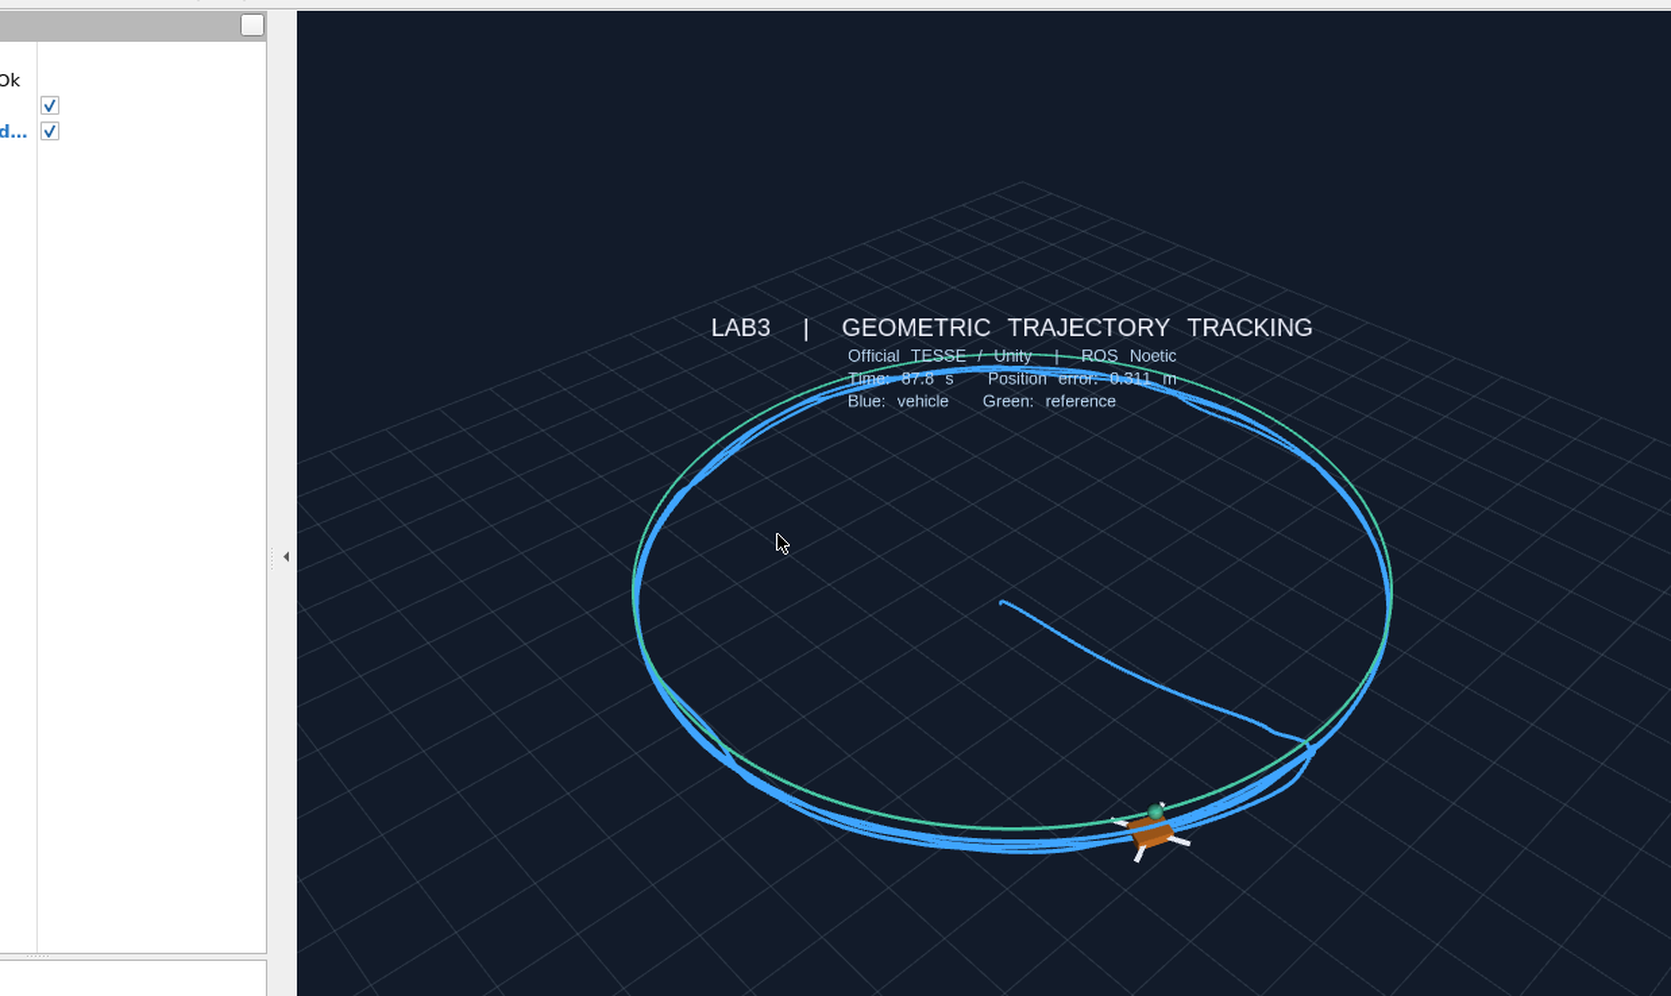
\includegraphics[width=\columnwidth]{figures/rviz_flight_cropped.png}
\caption{RViz during closed-loop flight. Green denotes the reference circle and blue denotes the trajectory reconstructed from official Unity odometry.}\label{fig:rviz_flight}
\end{figure}

Figure~\ref{fig:rviz_flight} shows the earlier RViz demonstration. Table~\ref{tab:ros} compares the initial Unity recording with the independently measured re-flight.

\section{DISCUSSION}
\subsection{What Each Design Choice Changes}
The comparisons separate three mechanisms. Smooth timing reduces the mismatch between an initially stationary vehicle and a moving reference; its strongest benefit appears at startup. Velocity damping governs oscillation and settling after that mismatch. Drag feedforward reduces the sustained feedback offset needed to oppose aerodynamic resistance. These effects appear in different portions of the same error history, which is why startup maxima and steady-state RMSE are reported together.

The ideal translational model provides a useful first explanation, but the attitude loop determines how quickly the required force direction can be realized. The residual periodic position error and the measured yaw lag both reveal that finite attitude response. Across three attitude-gain settings, the near-yaw balance predicts the measured heading offset within $0.20^\circ$, linking the numerical result to the angular-rate damping term.

\subsection{ROS Flight Residual and Altitude Regulation}
In the initial flight the vehicle flew an average of 0.249 m below the reference. The archived retuned flight reported a position RMSE of 0.0107 m at a median state interval of 0.020 s. With the same delivered gains, the independent re-flight yielded \FlightPos\ m at a median state interval of \FlightDt\ s. Its mean height bias was \FlightBias\ m and its height RMSE was \FlightHeight\ m. The two recordings differ in feedback timing, so their errors characterize the full closed loop rather than the gain change alone. In this re-flight, the smaller mean altitude offset coexisted with larger height oscillations and substantial horizontal error.

\subsection{Directions for Improving the Controller}
A natural next step is to compute desired angular velocity from $\widehat\Omega_d=R_d^T\dot R_d$ and use the moving-attitude rate error
\begin{equation}
e_\Omega=\Omega-R^TR_d\Omega_d.
\end{equation}
The full geometric moment law then includes the corresponding rate and angular-acceleration feedforward terms\cite{lee}. This directly targets the heading-lag mechanism identified in the present experiment. A subsequent comparison should retain the same circle, timing law, and drag conditions so that the effect of the attitude terms can be measured separately.

For actuator-constrained flight, trajectory timing should also account for feasible rotor inputs. The large peak commands during direct startup indicate why smooth references are valuable beyond reducing tracking error. Introducing motor dynamics and bounded rotor speeds would make the timing-versus-input tradeoff an explicit part of the planning problem.

\section{TEAM WORK ALLOCATION}
The five members shared responsibility for the project, with each contributing 20\% of the overall work. Table~\ref{tab:contributions} lists the main responsibility of each member.

\begin{table}[tbp]
\caption{Team responsibilities and equal contribution}\label{tab:contributions}
\centering\footnotesize\setlength{\tabcolsep}{3pt}
\begin{tabularx}{\columnwidth}{@{}lYr@{}}
\toprule
Member & Responsibility & Share\\\midrule
Li Shuyu & Trajectory planning and flight tests & 20\%\\
Deng Chengyang & Controller and gain tuning & 20\%\\
Zhou Jingxin & Unity--ROS integration and tests & 20\%\\
Zhou Chunyang & Flight logs and error analysis & 20\%\\
Zhang Yuxin & Visualization and report review & 20\%\\
\bottomrule
\end{tabularx}
\end{table}

\subsection{Individual Contribution of Li Shuyu}
I was responsible for trajectory planning and flight testing, with work extending from the analytical reference to its execution in the integrated ROS--Unity system. The trajectory specifies the position, velocity, acceleration and tangent heading that the controller must realize at every instant. My work on the circular path and its time parameterization defined the flight task, the required motion derivatives and the startup demands used to evaluate the controller. The resulting reference included the 5 m radius, 2 m altitude, cruise-speed settings, acquisition hold and smooth phase-speed transition. These elements established a common flight task for the team's control, integration and measurement work.

My trajectory-design work addressed the large transient created when a stationary vehicle receives a moving reference. I compared direct startup with a smooth transition using position error, peak tilt and rotor-speed demand. In the matched no-drag experiment, smooth timing reduced peak startup error from \NomStart\ m to \SmoothStart\ m, a \StartGain\% reduction, and peak tilt from \NomTilt$^\circ$ to \SmoothTilt$^\circ$. This comparison tied a specific planning decision to measured tracking performance. I also examined cruise speeds of 1.25, 2.5 and 5 m/s to relate lap time to centripetal acceleration and tracking error. Together, these experiments supplied a quantitative basis for selecting the startup schedule and cruise speed used in flight testing.

I also carried responsibility for testing whether the integrated system could execute the planned trajectory. Working with the control and simulator-integration teammates, I checked acquisition of the starting waypoint, entry into circular motion and completion of the orbit. I compared the commanded and observed paths in RViz and used the recorded results to assess execution under the tested conditions. The new flight covered \FlightLaps\ revolutions and recorded a position RMSE of \FlightPos\ m. Evaluating the full flight exposed the effect of irregular state updates on trajectory execution, including the gap between the numerical tracking response and the measured Unity flight. My contribution therefore connected three stages of the experiment, the construction of the reference, the controlled comparison of timing choices and the assessment of the integrated system in flight. I documented these planning decisions and flight observations so that the team's implementation could be evaluated against an explicit, repeatable task.

\balance
\section{CONCLUSIONS}
The standard allocation matrix has rank four. Reversing rotors 3 and 4 reduces its rank to three and couples pitch and yaw. Across fourteen numerical conditions, smooth timing reduces startup error, drag compensation reduces steady tracking offset, and the ratio of attitude gains accounts for the observed heading lag. With both timing and compensation, peak startup error is \JointStart\ m and steady-state RMSE is \JointSteady\ m under drag. After the force pulse, tracking returns to within one centimeter of the unperturbed trajectory in 2.17 s. The new Unity flight covered \FlightLaps\ laps at a commanded 1.25 m/s. Sample-weighted and time-weighted position RMSE were \FlightPos\ m and \FlightTimePos\ m. Radial and heading RMSE were \FlightRad\ m and \FlightYaw$^\circ$, respectively.


\begin{thebibliography}{9}
\bibitem{lab} MIT SPARK, \href{https://vnav.mit.edu/labs_2023/lab3/exercises.html}{Visual Navigation for Autonomous Vehicles: Lab 3 Exercises} 2023.
\bibitem{tf2} ROS, \href{https://github.com/ros/geometry2/tree/noetic-devel}{geometry2: tf2 and tf2\_geometry\_msgs} noetic-devel.
\bibitem{eigen} Eigen, \href{https://libeigen.gitlab.io/eigen/docs-nightly/group__Geometry__Module.html}{Quaternion and geometry module documentation}.
\bibitem{lee} T. Lee, M. Leok, and N. H. McClamroch, ``Geometric tracking control of a quadrotor UAV on SE(3),'' in \emph{Proc. IEEE Conf. Decision and Control}, 2010, pp. 5420--5425, doi: 10.1109/CDC.2010.5717652.
\bibitem{code} MIT SPARK, \href{https://github.com/MIT-SPARK/VNAV-labs/releases/tag/VNAV2021}{VNAV-labs: VNAV2021 release}.
\end{thebibliography}
\end{document}
